%%%%%%%%%%%%%%%%%%%%%%%%%%%%%%%%%%%%%%%%%
% Structured General Purpose Assignment
% LaTeX Template
%
% Template Name: Anthony
% The template was named after my friend Anthony.
% Strong inspired by Apache Hadoop and Java (programming language)
%
% Author: Ang LEE
%
% Blog: http://angli.me/
%
% Github: https://github.com/leeang/
%
%%%%%%%%%%%%%%%%%%%%%%%%%%%%%%%%%%%%%%%%%

%----------------------------------------------------------------------------------------
%	CONSTANTS
%----------------------------------------------------------------------------------------

\newcommand{\hmwkTitle}{Report \#2}						% Assignment title
\newcommand{\hmwkClass}{Power System Analysis}			% Course name
\newcommand{\hmwkClassTime}{}							% Workshop time
\newcommand{\hmwkClassInstructor}{}						% Tutor name
\newcommand{\hmwkAuthorName}{Ang LEE}					% Student name

\newcommand{\hmwkGraphicsPath}{img/}					% Graphics path
\newcommand{\hmwkCodePath}{code}						% Code path

%----------------------------------------------------------------------------------------
%	TEMPLATE
%----------------------------------------------------------------------------------------

\documentclass{article}

\usepackage{fancyhdr}	% Required for custom headers
\usepackage{lastpage}	% Required to determine the last page for the footer
\usepackage{extramarks} % Required for headers and footers
\usepackage{graphicx}	% Required to insert images
\graphicspath{\hmwkGraphicsPath}

\usepackage{float}
\usepackage{epstopdf}	% Required to insert .eps images
\usepackage{amssymb}
\usepackage{amsmath}
% \usepackage[hidelinks]{hyperref}

% MATLAB syntax highlighting
\usepackage{color}		% Required to define colors
\definecolor{commentColor}{RGB}{34,139,34}
\definecolor{stringColor}{RGB}{160,32,240}
\usepackage{listings}
\lstset{
	language=Matlab,
	basicstyle=\footnotesize\ttfamily,
	keywordstyle=\color{blue},
	stringstyle=\color{stringColor},
	commentstyle=\usefont{T1}{pcr}{m}{n}\color{commentColor},
	tabsize = 4,
	breaklines=true,
	showstringspaces=false,
	numbers=left,
	numberstyle=\scriptsize,
	firstnumber=1,
	numberfirstline=true,
	stepnumber=5,
	frame=leftline
}

% change \textbf textbf
\definecolor{bfcolor}{RGB}{221,75,57}
\DeclareTextFontCommand{\textbf}{\bfseries\color{bfcolor}}

% change \texttt color
\definecolor{ttcolor}{RGB}{0,103,179}
\DeclareTextFontCommand{\texttt}{\ttfamily\color{ttcolor}}

% change headings color
\usepackage{sectsty}
\definecolor{sectioncolor}{RGB}{0,102,33}
\sectionfont{\color{sectioncolor}\sffamily}
\definecolor{subsectioncolor}{RGB}{26,131,171}
\subsectionfont{\color{subsectioncolor}\sffamily}
\definecolor{subsubsectioncolor}{RGB}{0,51,102}
\subsubsectionfont{\color{subsubsectioncolor}\sffamily}

% Margins
\topmargin=-0.45in
\evensidemargin=-0.3in
\oddsidemargin=-0.3in
\textwidth=7.1in
\textheight=9.0in
\headsep=0.25in

\linespread{1.1}		% Line spacing

% Set up the header and footer
\pagestyle{fancy}
\lhead{\hmwkTitle} % Header Left 
\chead{} % Header Center
\rhead{\hmwkClass} % Header Right
\lfoot{628305 Fei CAO, 629636 Qi SUN, 631317 Ang LI} % Footer Left
\cfoot{} % Footer Center
\rfoot{Page\ \thepage\ of\ \pageref{LastPage}} % Footer Right
\renewcommand\headrulewidth{0.4pt} % Size of the header rule
\renewcommand\footrulewidth{0.4pt} % Size of the footer rule

\setlength\parindent{0pt} % Removes all indentation from paragraphs

%----------------------------------------------------------------------------------------
%	Problem and Section
%----------------------------------------------------------------------------------------

\newenvironment{homeworkProblem}[1]{
	\section*{#1}
	}{
}
\newenvironment{homeworkSection}[1]{
	\subsection*{#1}
	}{
}
\newcommand{\problemAnswer}[1]{
	\noindent\framebox[\columnwidth][c]{
		\begin{minipage}{0.98\columnwidth}
			#1
		\end{minipage}
	}
}

%----------------------------------------------------------------------------------------
%	Document
%----------------------------------------------------------------------------------------

\begin{document}

\section*{Pre-workshop Calculations}

\subsection*{1.}
\begin{equation}\label{eq1}
\Big( 2 P_{D_{cr}} (G_{line} - \beta B_{line}) - |Y_{line}|^2 |V_1|^2 \Big)^2 - 4 |Y_{line}|^2 P_{D_{cr}}^2 (1 + \beta^2) = 0
\end{equation}

We have known
\begin{align*}
Z_{line} = (0.01 + j0.5)
\Longrightarrow Y_{line} = 0.04 - j1.9992
\Longrightarrow
\begin{cases}
G_{line} = 0.04 \text{ pu}\\
B_{line} = -1.9992 \text{ pu}
\end{cases}
\end{align*}
\begin{align*}
|V_1| &= 1 \text{ pu}\\
\end{align*}

For known $\beta$, Eq. \ref{eq1} can be sovled.
\begin{align*}
P_{D_{cr}} =
\begin{cases}
0.9801999800 \text{ pu} &pf = 0\\
0.4949882502 \text{ pu} &pf = 0.8 \text{ lagging}\\
1.9221529035 \text{ pu} &pf = 0.8 \text{ leading}
\end{cases}
\end{align*}

\begin{equation}\label{eq2}
|V_{2_{cr}}|^2 = \frac{|Y_{line}|^2 |V_1|^2 - 2 P_{D_{cr}} (G_{line} - \beta B_{line})}{2 |Y_{line}|^2}
\end{equation}
Evaluate $|V_{2_{cr}}|$ via Eq. \ref{eq2}
\begin{align*}
|V_{2_{cr}}| =
\begin{cases}
0.700141 \text{ pu} &pf = 0\\
0.556264 \text{ pu} &pf = 0.8 \text{ lagging}\\
1.096169 \text{ pu} &pf = 0.8 \text{ leading}
\end{cases}
\end{align*}

\subsection*{2.}
\begin{equation}\label{eq3}
|V_2|^4 |Y_{line}|^2 + |V_2|^2 \Big(2 P_D (G_{line} - \beta B_{line}) - |Y_{line}|^2 |V_1|^2 \Big) + P_D^2 (1+\beta^2) = 0
\end{equation}
\begin{align*}
P_D = \lambda \cdot \frac{5}{50} \cdot pf = 0.1 \lambda \cdot pf
\end{align*}

We have known
\begin{align*}
pf = 1 &\Longrightarrow \beta = 0\\
\lambda &= 4\\
P_D &= 0.4
\end{align*}

Eq. \ref{eq3} can be solved
\begin{align*}
|V_2| =
\begin{cases}
0.9746 \text{ pu}\\
0.2053 \text{ pu}
\end{cases}
\end{align*}

\subsection*{3.}
We have known
\begin{align*}
pf = 0.8 \text{ lagging} &\Longrightarrow \beta = \frac{\sqrt{1 - pf^2}}{pf} = 0.75\\
P_D &= 0.1 \lambda \cdot pf = 0.32
\end{align*}

Eq. \ref{eq3} can be solved
\begin{align*}
|V_2| =
\begin{cases}
0.8343 \text{ pu}\\
0.2398 \text{ pu}
\end{cases}
\end{align*}

\subsection*{4.}
We have known
\begin{align*}
pf = 0.8 \text{ leading}&\Longrightarrow \beta = - \frac{\sqrt{1 - pf^2}}{pf} = -0.75\\
P_D &= 0.1 \lambda \cdot pf = 0.32
\end{align*}

Eq. \ref{eq3} can be solved
\begin{align*}
|V_2| =
\begin{cases}
1.0956 \text{ pu}\\
0.1826 \text{ pu}
\end{cases}
\end{align*}

%----------------------------------------------------------------------------------------
%	Experiment 1
%----------------------------------------------------------------------------------------

\section*{Experiment 1}

\subsection*{2. \& 3.}
\begin{figure}[H]
\centering
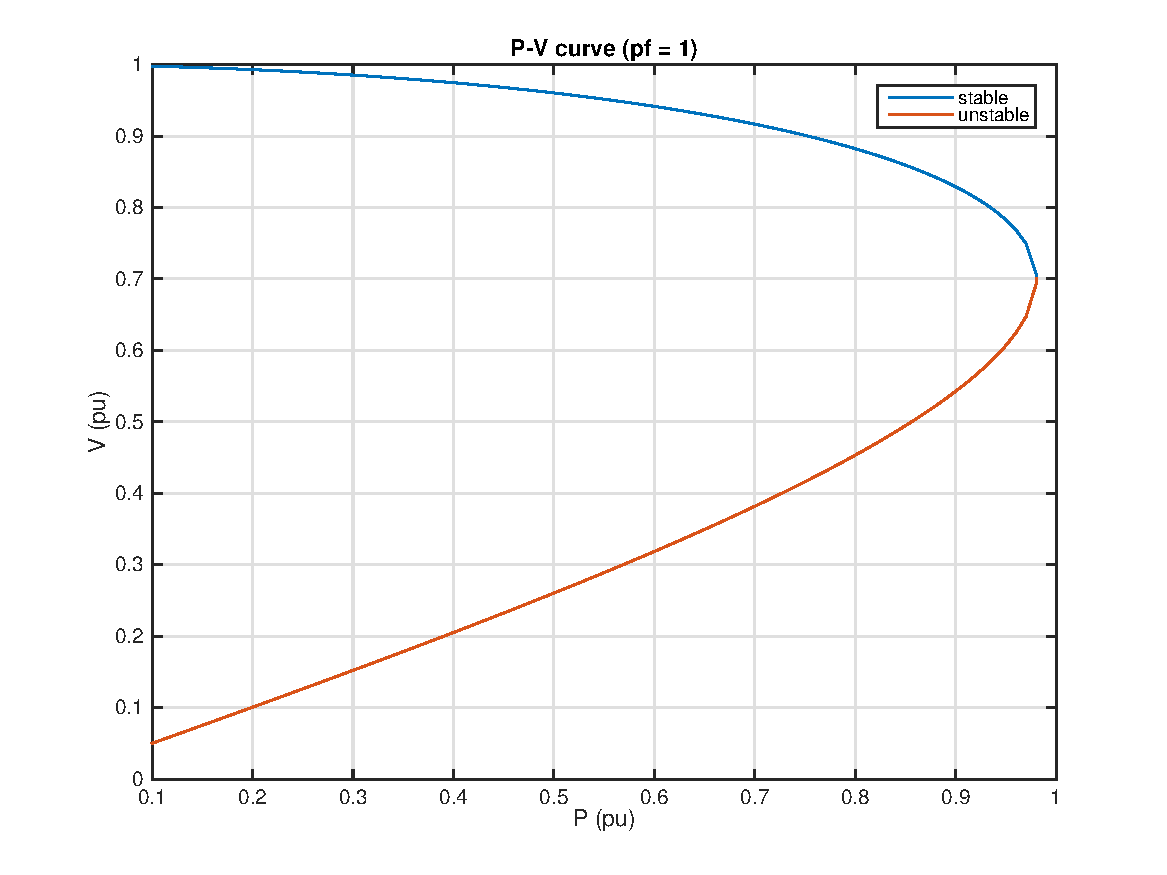
\includegraphics[width=0.5\linewidth]{e1_q2}
\caption{$P$ - $V$ curve when $pf$ = 0}
\end{figure}

\subsection*{4.}
\begin{figure}[H]
\centering
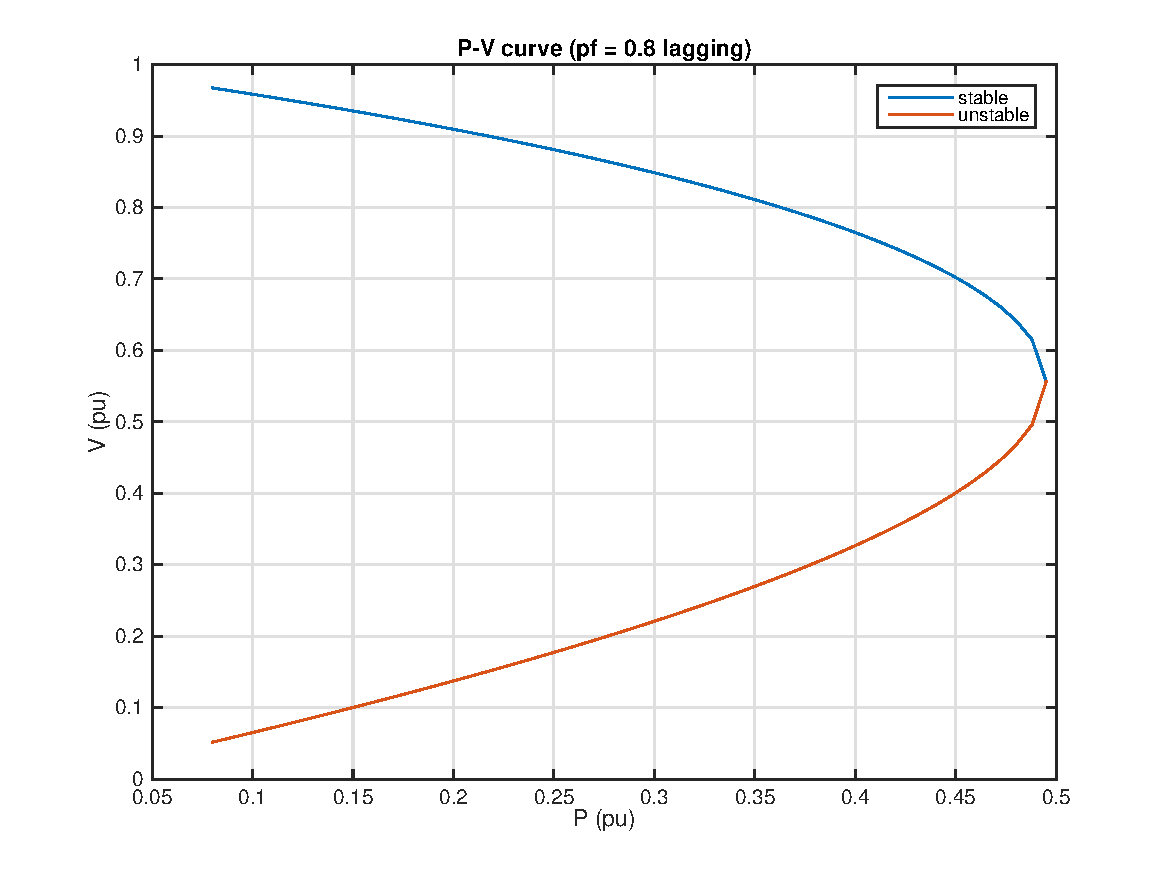
\includegraphics[width=0.5\linewidth]{e1_q4}
\caption{$P$ - $V$ curve when $pf$ = 0.8 lagging}
\end{figure}

\subsection*{5.}
\begin{figure}[H]
\centering
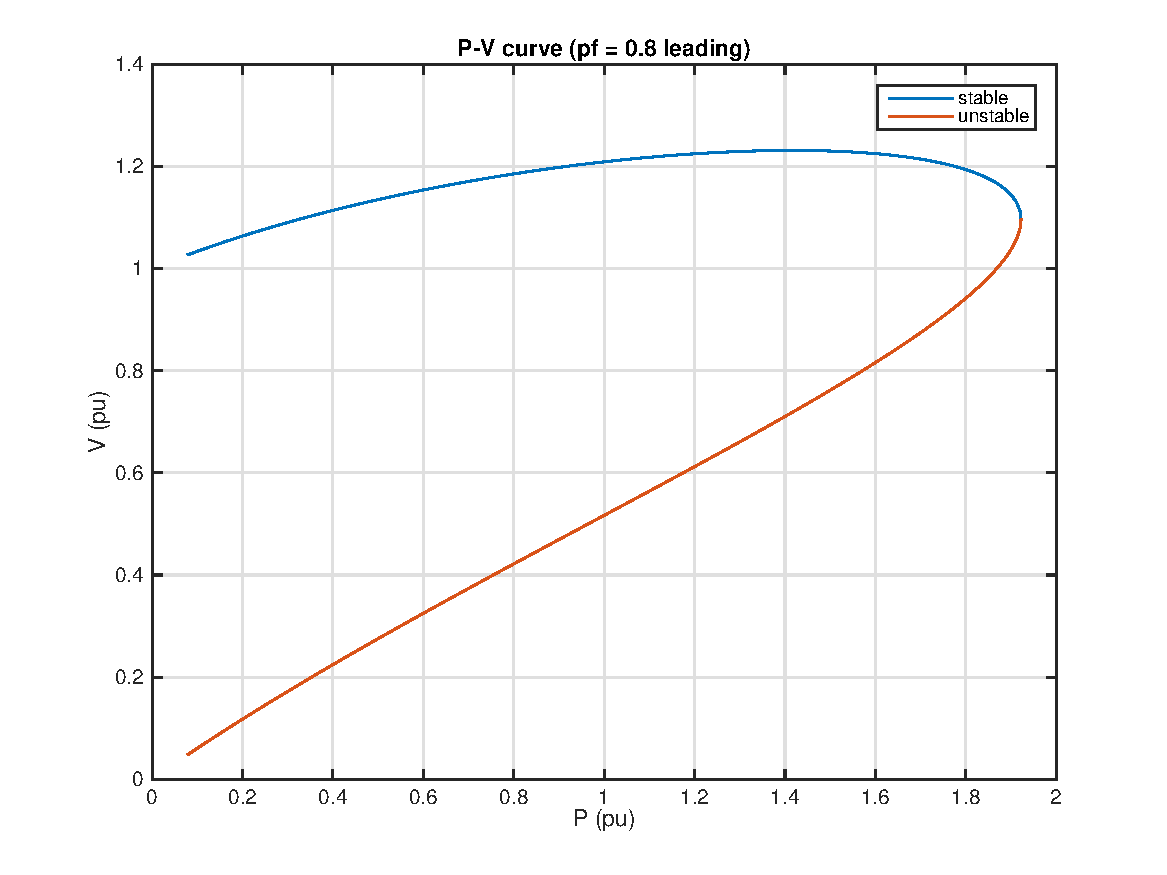
\includegraphics[width=0.5\linewidth]{e1_q5}
\caption{$P$ - $V$ curve when $pf$ = 0.8 leading}
\end{figure}

%----------------------------------------------------------------------------------------
%	Experiment 2
%----------------------------------------------------------------------------------------

\section*{Experiment 2}

\subsection*{4.}
\begin{figure}[H]
\centering
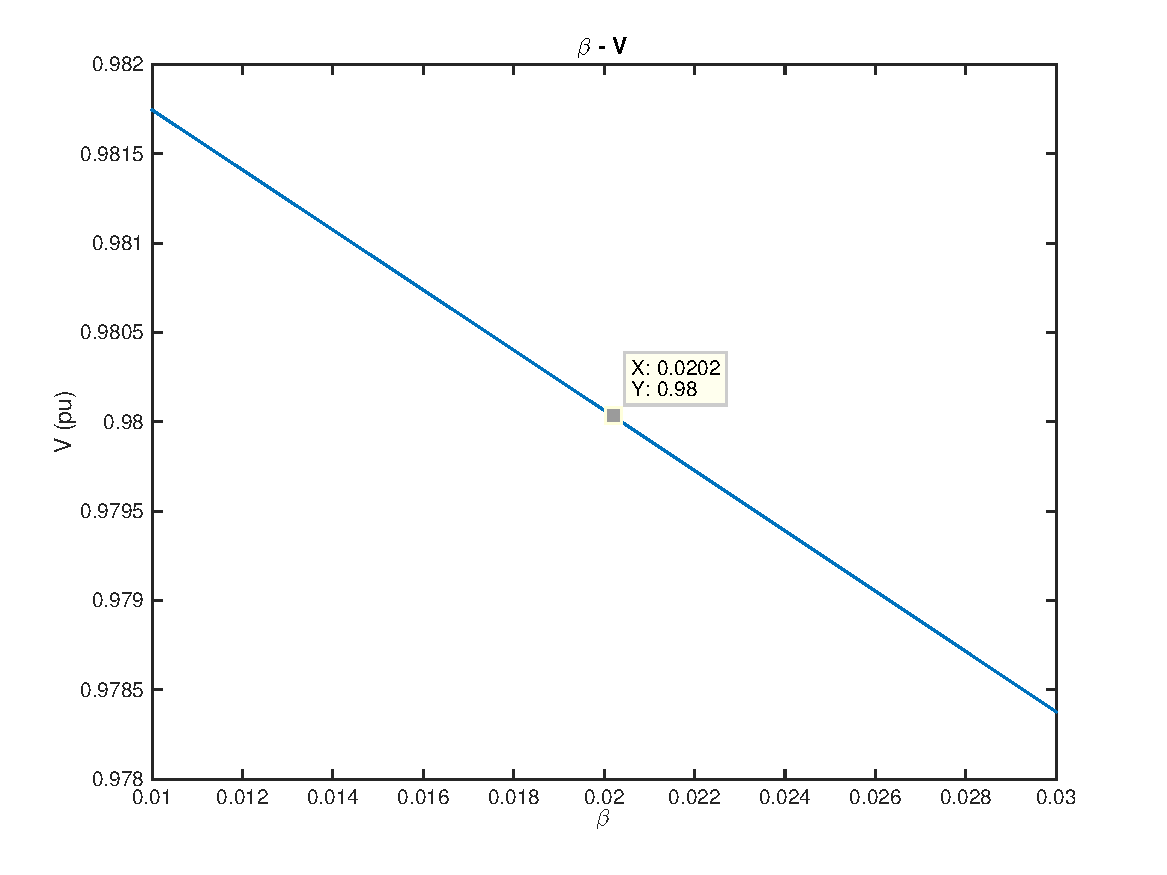
\includegraphics[width=0.5\linewidth]{e2_q4}
\caption{$\beta$ - $V$ curve}
\end{figure}

%----------------------------------------------------------------------------------------

\end{document}
